\chapter{Beispielkapitel}\label{chap:example} % \label used for referencing the chapter in text

\lipsum[]

Das hier gezeigte \gls{latex}-Beispiel soll einige Möglichkeiten aufzeigen, wie ein Dokument gestaltet werden kann.

Das \acrfull{tia}-Portal ist eine Programmierumgebung, die speziell für die Projektierung von Siemens-Steuerungen entwickelt wurde. Im nachfolgenden wird die Abkürzung \acrshort{tia} aus Gründen der Lesbarkeit verwendet.

\begin{mycapequ}[!ht]
    \begin{equation}
        {P(\bigcup_{n=1}^n A_n) \leq \sum_{n=1}^n P(A_n)}
        \label{eq:bool} %\label used for referencing the equation in text
    \end{equation}
    \caption{Bool'sche Gleichung}
\end{mycapequ}

\noindent \cref{eq:bool} zeigt eine Gleichung in \gls{latex}.

\clearpage

\begin{figure}[!ht]
    \centering
    \includegraphics[width=1.0\textwidth]{example-image-a}
    \captionsetup{width=1.0\textwidth}
    \caption[skalierte Beispielabbildung]{skalierte Beispielabbildung (eigene Abbildung)}
    \label{fig:scaledexampleimagea} % \label used for referencing the figure in text
\end{figure}

\begin{figure}[!ht]
\centering
    \begin{minipage}[c]{.475\textwidth}
    \centering
        \includegraphics[width=1.0\linewidth]{example-image-b}
        \captionof{figure}[Beispielabbildung b]{Beispielabbildung b (eigene Abbildung)}
        \label{fig:horizontalalignedimageb} % \label used for referencing the figure in text
    \end{minipage}\hspace{.025\textwidth}
    \begin{minipage}[c]{.475\textwidth}
        \centering
        \includegraphics[width=1.0\linewidth]{example-image-c}
        \captionof{figure}[Beispielabbildung c]{Beispielabbildung c (eigene Abbildung)}
        \label{fig:horizontalalignedimagec} % \label used for referencing the figure in text
    \end{minipage}
\end{figure}

\noindent Oben sind einige Beispielabbildungen mit verschiedenen Skalierungen zu erkennen.

Außerdem besteht die Möglichkeit den Text, um ein Bild herum anzuordnen. Das sieht wie folgt aus.

\lipsum[1]

\begin{wrapfigure}{l}{0.4\textwidth}
    \centering
    \includegraphics[width=0.9\linewidth]{example-image}
    \captionsetup{width=0.9\linewidth}
    \caption[Beispielabbildung mit Text umrandet]{Beispielabbildung mit Text umrandet (eigene Abbildung)}
    \label{fig:textwrappedaroundexampleimage} % \label used for referencing the figure in text
\end{wrapfigure}

\lipsum[2-4]

\clearpage

\section{Beispielabschnitt}\label{sec:example} % \label used for referencing the section in text

\begin{table}[!ht]
    \centering
        \begin{tabular}{ | c | c | c | }
            \hline
            symbol & value & unit \\ \hline            
            $z Na$ & 11 & - \\ \hline      
            $z F$ & 9 & - \\ \hline      
            $Emax Na$ & 0.545 & $[MeV]$ \\ \hline
        \end{tabular}
        \caption{Beispieltabelle}
        \label{tab:example} % \label used for referencing the table in text
\end{table}

\noindent Hier (s.\cref{tab:example}) lässt sich eine kleine Beispieltabelle, die mit LaTeX erstellt wurde erkennen.

\clearpage

\section{Letzter Abschnitt}\label{sec:last} % \label used for referencing the section in text

\cref{fig:tikzexamplegraphics} zeigt eine Beispielgrafik, die mit dem Paket \glqq Tikz\grqq{} erstellt wurde.

\begin{figure}[!ht]
    \centering
	\begin{tikzpicture}
        \draw (0,0) circle (1);
        \draw (2,0) circle (1.5in);
        \draw (5,0) ellipse (10pt and 20 pt);
        \draw node at (3,0) {$f(x)$};
        \filldraw (6,0) circle (0.1cm) node[anchor=west]{Anchored Node};
    \end{tikzpicture}
    \caption{Tikz Beispielgrafik}
    \label{fig:tikzexamplegraphics} % \label used for referencing the figure in text
\end{figure}

\noindent Als ein weiteres komplexeres Beispiel kann hier auch noch folgende \cref{fig:tikzexamplediagram} angeführt werden.

\begin{figure}[!ht]
    \centering
    \begin{tikzpicture}[
                        youngnode/.style={rectangle, draw=red!60, fill=red!5, very thick, minimum size=40},
                        oldnode/.style={rectangle, draw=blue!60, fill=blue!5, very thick, minimum size=40},
                        ]
        %Nodes
        \node[oldnode]        (SusO)                            { $S_O(t)$};
        \node[oldnode]        (InfO)       [below=of SusO]      { $I_O(t)$};
        \node[oldnode]        (RecO)       [below=of InfO]      { $R_O(t)$};

        \node[youngnode]      (SusY)        [left=of SusO]      { $S_Y(t)$};
        \node[youngnode]      (InfY)        [left=of InfO]      { $I_Y(t)$};
        \node[youngnode]      (RecY)        [left=of RecO]      { $R_Y(t)$};

        %Lines
        \draw[->, very thick] (SusO.south east)  to node[right] {$a_{OO}$} (InfO.north east);
        \draw[->, very thick] (InfO.south)  to node[right] {$b_O$} (RecO.north);
        \draw[->, very thick] (RecO.east)  .. controls  +(right:17mm) and +(right:17mm)   .. (SusO.east);

        \draw[->, very thick] (SusY.south west)  to node[left] {$a_{YY}$} (InfY.north west);
        \draw[->, very thick] (InfY.south)  to node[left] {$b_Y$} (RecY.north);
        \draw[->, very thick] (RecY.west) .. controls  +(left:17mm) and +(left:17mm)   .. (SusY.west);

        \draw[dashed,->, very thick] (InfO.north west)  to  (SusY.south east);
        \draw[->, very thick] (SusY.south east)  to node[left] {$a_{OY}$} (InfY.north east);

        \draw[->, very thick] (SusO.south west)  to node[right] {$a_{YO}$} (InfO.north west);
        \draw[dashed,->, very thick] (InfY.north east)  to  (SusO.south west);
    \end{tikzpicture}
    \caption{Tikz Beispieldiagramm}
    \label{fig:tikzexamplediagram} % \label used for referencing the figure in text
\end{figure}

\clearpage

\noindent Das Paket \glqq pgfplots\grqq{} basiert auf \glqq Tikz\grqq{} und ermöglicht das Zeichnen von mathematischen Diagrammen aller Art. In \cref{fig:pgfplotsexample2D} ist dies anhand eines Beispiels dargestellt.

\begin{figure}[!ht]
    \centering
    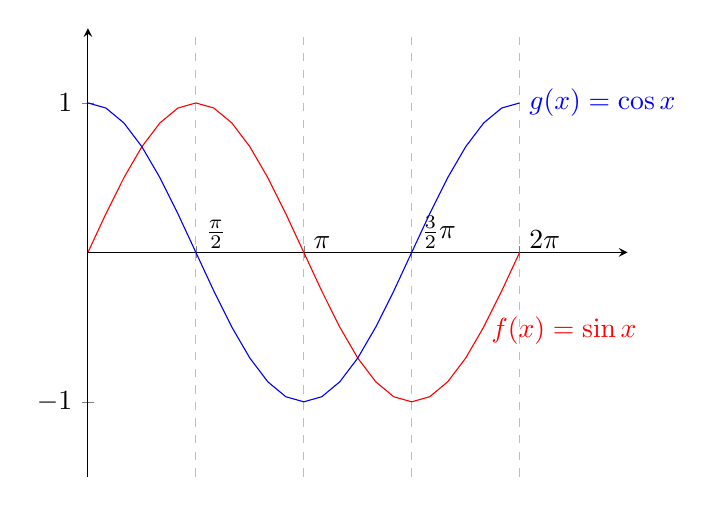
\begin{tikzpicture}
        \begin{axis}[clip=false,xmin=0,xmax=2.5*pi,ymin=-1.5,ymax=1.5, axis lines=middle,xtick={0,pi/2,pi,3*pi/2,2*pi},xticklabels={$0$,$\frac{\pi}{2}$,$\pi$,$\frac{3}{2}\pi$,$2\pi$},xticklabel style={anchor=south west},xmajorgrids=true,grid style=dashed]
            \addplot[domain=0:2*pi,red]{sin(deg(x))}
            node[right,pos=0.9]{$f(x)=\sin x$};
            \addplot[domain=0:2*pi,blue]{cos(deg(x))}
            node[right,pos=1.0]{$g(x)=\cos x$};
        \end{axis}
    \end{tikzpicture}
    \caption{pgfplots Beispiel einer 2D-Grafik}
    \label{fig:pgfplotsexample2D} % \label used for referencing the figure in text
\end{figure}

\noindent Außerdem können auch 3D-Grafiken damit erstellt werden, wie in \cref{fig:pgfplotsexample3D} und in \cref{fig:anotherpgfplotsexample3D} zu sehen ist.

\begin{figure}[!ht]
    \centering
    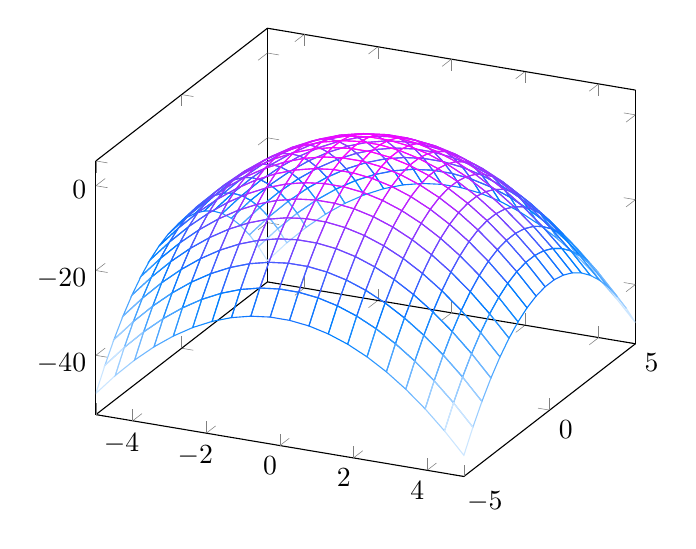
\begin{tikzpicture}
        \begin{axis}[colormap/cool]
            \addplot3[mesh,samples=20]{1-x^2-y^2};
        \end{axis}
    \end{tikzpicture}
    \caption{pgfplots Beispiel einer 3D-Grafik}
    \label{fig:pgfplotsexample3D} % \label used for referencing the figure in text
\end{figure}

\clearpage

\begin{figure}[!ht]
    \centering
    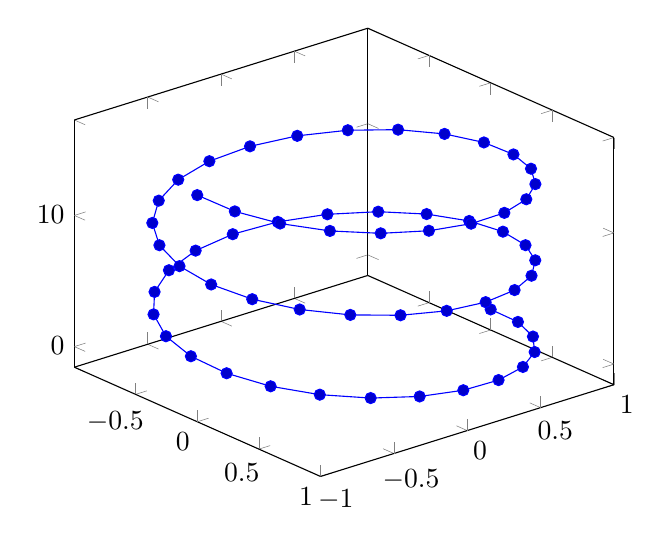
\begin{tikzpicture}
        \begin{axis}[view={50}{30}]
            \addplot3+[domain=0:5*pi,samples=60,samples y=0]({sin(deg(x)},{cos(deg(x)},{x});
        \end{axis}
    \end{tikzpicture}
    \caption{weiteres pgfplots Beispiel einer 3D-Grafik}
    \label{fig:anotherpgfplotsexample3D} % \label used for referencing the figure in text
\end{figure}

\noindent Darüber hinaus können auch Daten aus .txt-Dateien ausgelesen werden und eine Grafik überführt werden (s. \cref{fig:pgfplotsexampledata}).

\begin{figure}[!ht]
    \centering
    \begin{minipage}[t]{1.0\linewidth}
        \centering
        \begin{tikzpicture}
            \begin{axis}[xmin=0, xmax=32, xlabel=$k$, ylabel=$x_k$, ymin=0, ymax=1, ymajorgrids=true, xmajorgrids=true, width=0.95\linewidth]
                \addplot+[only marks] table[x=k, y=hk]{data/exampledata.txt};
            \end{axis}
        \end{tikzpicture}
        \caption{Beispiel einer Datenreihe mit pgfplot}
        \label{fig:pgfplotsexampledata} % \label used for referencing the figure in text
    \end{minipage}
\end{figure}

\noindent Weitere Informationen zu den Paketen gibt es in der Dokumentation unter \cite{tikz} und \cite{pgfplots}.